\let\negmedspace\undefined
\let\negthickspace\undefined
\documentclass[journal]{IEEEtran}
\usepackage[a5paper, margin=10mm, onecolumn]{geometry}
%\usepackage{lmodern} % Ensure lmodern is loaded for pdflatex
\usepackage{tfrupee} % Include tfrupee package

\setlength{\headheight}{1cm} % Set the height of the header box
\setlength{\headsep}{0mm}     % Set the distance between the header box and the top of the text

\usepackage{gvv-book}
\usepackage{gvv}
\usepackage{cite}
\usepackage{amsmath,amssymb,amsfonts,amsthm}
\usepackage{algorithmic}
\usepackage{graphicx}
\usepackage{textcomp}
\usepackage{xcolor}
\usepackage{txfonts}
\usepackage{listings}
\usepackage{enumitem}
\usepackage{mathtools}
\usepackage{gensymb}
\usepackage{comment}
\usepackage[breaklinks=true]{hyperref}
\usepackage{tkz-euclide} 
\usepackage{listings}
% \usepackage{gvv}                                        
\def\inputGnumericTable{}                                 
\usepackage[latin1]{inputenc}                                
\usepackage{color}                                            
\usepackage{array}                                            
\usepackage{longtable}                                       
\usepackage{calc}                                             
\usepackage{multirow}                                         
\usepackage{hhline}                                           
\usepackage{ifthen}                                           
\usepackage{lscape}
\begin{document}

\bibliographystyle{IEEEtran}
\vspace{3cm}
\title{1.1.3.6}
\author{AI24BTECH11012-Pushkar Gudla}
% \maketitle
% \newpage
{\let\newpage\relax\maketitle}

\renewcommand{\thefigure}{\theenumi}
\renewcommand{\thetable}{\theenumi}
\setlength{\intextsep}{10pt} % Space between text and floats


\numberwithin{equation}{enumi}
\numberwithin{figure}{enumi}
\renewcommand{\thetable}{\theenumi}

\textbf{Question:} If $\myvec{3\\3}$, $\myvec{6\\y}$, $\myvec{x\\7}$ and $\myvec{5\\6}$ are the vertices of a parallelogram taken in order, find the values of $x$ and $y$. 
		\hfill{(10, 2011)}\\

		\solution Property: midpoints of diagnol coincide. Let $\vec{O}$ be the midpoint of the diagnols. \\
		\begin{align}
			\vec{O} &=\frac{\myvec{3\\3}+\myvec{x\\7}}{2}\\
			\implies \vec{O} &= \myvec{\frac{3+x}{2}\\5}
			\text{, And we also have:}\\
			\vec{O} &= \frac{\myvec{6\\y}+\myvec{5\\6}}{2}\\
		\implies	\vec{O} &= \myvec{5.5\\\frac{6+y}{2}}\\
			\text{On comparing the two, we get, }
			x &= 8\\
			y &= 4
		\end{align}

\begin{figure}[H]
	\centering
	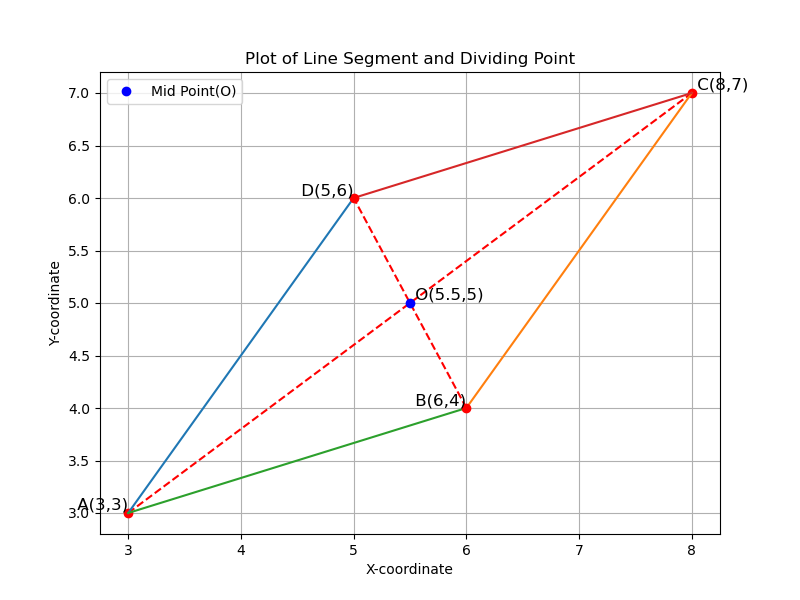
\includegraphics[scale=0.4]{figs/parallelogram.png}
	\label{Fig}
\end{figure}


\end{document}
